\chapter{Especificación de Casos de Uso}
A continuación se especifican los actores que harán uso del sistema con el fin de identificar todos los casos de uso a desarrollar y posteriormente se
expone una descripción tabulada de los casos de uso y diagramas para su mejor comprensión.\\

La notación tabular elegida es la siguiente:
\begin{table}[!ht] %% Tabla Especificación de casos de uso.
   \centering
   \begin{tabular}{|p{4cm}|p{11.5cm}|}
      \hline
      \textbf{Caso de uso} & \textit{Nombre del caso de uso.}\\ \hline
      \textbf{Objetivo} & \textit{Objetivo principal del caso de uso.}\\ \hline
      \textbf{Actores} & \textit{Actores implicados en el caso de uso.}\\ \hline
      \textbf{Disparador} & \textit{Descripción de la acción que provoca la ejecución del caso de uso.}\\ \hline
      \textbf{Precondiciones} & \textit{Condiciones que se deben de dar para la ejecución del caso de uso.}\\ \hline
      \textbf{Descripción} & \textit{Breve descripción del comportamiento del caso de uso.}\\ \hline
      \multicolumn{2}{|c|}{\textbf{Curso normal de los eventos}}\\ \hline
   \end{tabular}
   \begin{tabular}{|p{7.75cm}|p{7.75cm}|}
      \hspace{2cm}\textbf{Acción de los actores} & \hspace{1.75cm}\textbf{Respuesta del sistema}\\ \hline
      \textit{Acciones que realizan los actores del caso de uso.} & \textit{Acciones que realiza el sistema.}\\ \hline
   \end{tabular}
   \begin{tabular}{|p{15.9cm}|}
      \hspace{6cm}\textbf{Cursos alternativos}\\ \hline
      \textit{Acciones a realizar fuera del curso normal de eventos.}\\ \hline
   \end{tabular}
   \caption{Modelo para la Especificación de Casos de Uso.}
\end{table}

   \section{Identificación de actores}
   Nuestro sistema sólo contará con un actor, que será el usuario del mismo y podrá realizar todas las operaciones disponibles.\\
   \begin{figure} [H] \begin{center}
      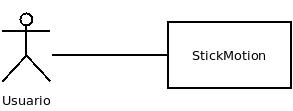
\includegraphics[width=0.5\textwidth]{./imagenes/actores}\label{actores}
      \caption{Identificación de actores.}
   \end{center} \end{figure}

   
   \section{Casos de Uso}
   El siguiente diagrama muestra los casos de uso identificados que se desarrollan.\\
   \begin{figure} [H] \begin{center}
      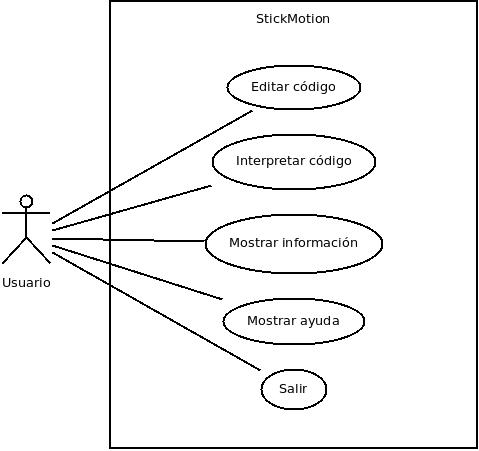
\includegraphics[width=0.7\textwidth]{./imagenes/dcu}\label{dcu}
      \caption{Diagrama de Casos de Uso.}
   \end{center} \end{figure}

   \begin{table}[!ht] %% Tabla Caso de uso 1 - Editar código.
      \centering
      \begin{tabular}{|p{4cm}|p{11.5cm}|}
         \hline
         \textbf{Caso de uso} & \textit{Editar código.}\\ \hline
         \textbf{Objetivo} & \textit{Editar el código a interpretar.}\\ \hline
         \textbf{Actores} & \textit{Usuario.}\\ \hline
         \textbf{Disparador} & \textit{Este caso de uso es disparado cada vez que el usuario realiza alguna modificación sobre
                                 el código a interpretar.}\\ \hline
         \textbf{Precondiciones} & \textit{Ninguna.}\\ \hline
         \textbf{Descripción} & \textit{El usuario edita el código a interpretar.}\\ \hline
         \multicolumn{2}{|c|}{\textbf{Curso normal de los eventos}}\\ \hline
    \end{tabular}
    \begin{tabular}{|p{7.75cm}|p{7.75cm}|}
      \hspace{2cm}\textbf{Acción de los actores} & \hspace{1.75cm}\textbf{Respuesta del sistema}\\ \hline
            & \textit{1.- El sistema da la posibilidad de editar el código mediante:}
                     \begin{itemize}
                        \item \textit{Abrir fichero.}
                        \item \textit{Guardar fichero.}
                        \item \textit{Escribir.}
                        \item \textit{Nuevo documento.}
                     \end{itemize} \\ \hline
    \end{tabular}
    \begin{tabular}{|p{15.9cm}|}
      \hspace{6cm}\textbf{Cursos alternativos}\\ \hline
      \textit{Ninguno.}\\ \hline
    \end{tabular}
    \caption{Caso de uso 1.- Editar código.}
   \end{table} 
   \begin{figure} [H] \begin{center}
      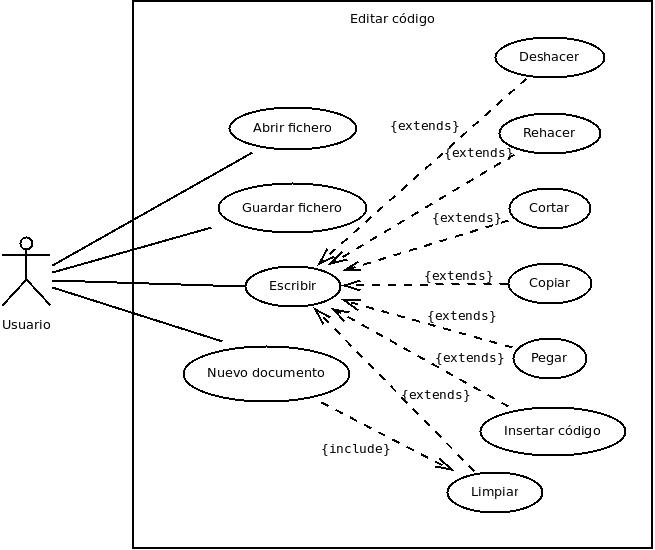
\includegraphics[width=0.9\textwidth]{./imagenes/cu1}\label{actores}
      \caption{Caso de uso 1.- Editar código.}
   \end{center} \end{figure}


   \begin{table}[!ht] %% Tabla Caso de uso 1.1 - Abrir fichero.
      \centering
      \begin{tabular}{|p{4cm}|p{11.5cm}|}
         \hline
         \textbf{Caso de uso} & \textit{Abrir fichero.}\\ \hline
         \textbf{Objetivo} & \textit{Abrir un fichero de texto con código Sticky.}\\ \hline
         \textbf{Actores} & \textit{Usuario.}\\ \hline
         \textbf{Disparador} & \textit{Este caso de uso se dispara cuando el usuario selecciona la opción correspondiente para abrir
                                 un fichero.}\\ \hline
         \textbf{Precondiciones} & \textit{Ninguna.}\\ \hline
         \textbf{Descripción} & \textit{El sistema abre un archivo de texto con código Sticky.}\\ \hline
         \multicolumn{2}{|c|}{\textbf{Curso normal de los eventos}}\\ \hline
    \end{tabular}
    \begin{tabular}{|p{7.75cm}|p{7.75cm}|}
      \hspace{2cm}\textbf{Acción de los actores} & \hspace{1.75cm}\textbf{Respuesta del sistema}\\ \hline
      \textit{1.- El usuario selecciona un fichero para abrir de sus sistema de ficheros.} & \textit{2.- El sistema comprueba el fichero.}
                                                                           \textit{3.- El sistema carga el fichero.}
                                                                           \textit{4.- El sistema limpia el editor y muestra la información
                                                                                       contenida en el fichero cargado.} \\ \hline
    \end{tabular}
    \begin{tabular}{|p{15.9cm}|}
      \hspace{6cm}\textbf{Cursos alternativos}\\ \hline
      \textit{2a.- El fichero no tiene extensión .stk}
         \textit{  2a1.- El sistema finaliza este caso de uso.} \\ \hline
    \end{tabular}
    \caption{Caso de uso 1.1.- Abrir fichero.}
   \end{table}


   \begin{table}[!ht] %% Tabla Caso de uso 1.2 - Guardar fichero.
      \centering
      \begin{tabular}{|p{4cm}|p{11.5cm}|}\hline
      \textbf{Caso de uso} & \textit{Guardar fichero.}\\ \hline
      \textbf{Objetivo} & \textit{Guarda un fichero con código Sticky.}\\ \hline
      \textbf{Actores} & \textit{Usuario.}\\ \hline
      \textbf{Disparador} & \textit{Este caso de uso se dispara cuando el usuario selecciona la opción correspondiente para guardar
                              un fichero.}\\ \hline
      \textbf{Precondiciones} & \textit{Ninguna.}\\ \hline
      \textbf{Descripción} & \textit{El sistema guarda un archivo de texto con código Sticky.}\\ \hline 
      \multicolumn{2}{|c|}{\textbf{Curso normal de los eventos}}\\ \hline
    \end{tabular}
    \begin{tabular}{|p{7.75cm}|p{7.75cm}|}
      \hspace{2cm}\textbf{Acción de los actores} & \hspace{1.75cm}\textbf{Respuesta del sistema}\\ \hline
      \textit{1.- El usuario selecciona la ruta y el nombre del fichero.} & \textit{2.- El sistema almacena el fichero.} \\ \hline
    \end{tabular}
    \begin{tabular}{|p{15.9cm}|}
      \hspace{6cm}\textbf{Cursos alternativos}\\ \hline
      \textit{2a.- El fichero no puede ser almacenado.}
      \textit{  2a1.- El sistema finaliza este caso de uso.} \\ \hline
    \end{tabular}
    \caption{Caso de uso 1.2.- Guardar fichero.}
   \end{table}


   \begin{table}[!ht] %% Tabla Caso de uso 1.3 - Escribir.
      \centering
      \begin{tabular}{|p{4cm}|p{11.5cm}|}
      \hline
         \textbf{Caso de uso} & \textit{Escribir.}\\ \hline
         \textbf{Objetivo} & \textit{Escribir código Sticky en el editor.}\\ \hline
         \textbf{Actores} & \textit{Usuario.}\\ \hline
         \textbf{Disparador} & \textit{Este caso de uso se dispara cuando el usuario realiza alguna operación sobre el editor.}\\ \hline
         \textbf{Precondiciones} & \textit{Ninguna.}\\ \hline 
         \textbf{Descripción} & \textit{Modifica el contenido del editor de código.}\\ \hline
         \multicolumn{2}{|c|}{\textbf{Curso normal de los eventos}}\\ \hline
    \end{tabular}
    \begin{tabular}{|p{7.75cm}|p{7.75cm}|}
      \hspace{2cm}\textbf{Acción de los actores} & \hspace{1.75cm}\textbf{Respuesta del sistema}\\ \hline
      \textit{1.- El usuario modifica el código en el editor.} &  \\ \hline
    \end{tabular}
    \begin{tabular}{|p{15.9cm}|}
      \hspace{6cm}\textbf{Cursos alternativos}\\ \hline     
      \textit{Ninguno.} \\ \hline
    \end{tabular}
    \caption{Caso de uso 1.3.- Escribir.}
   \end{table}


   \begin{table}[!ht] %% Tabla Caso de uso 1.4 - Deshacer.
      \centering
      \begin{tabular}{|p{4cm}|p{11.5cm}|}
      \hline
      \textbf{Caso de uso} & \textit{Deshacer.}\\ \hline
      \textbf{Objetivo} & \textit{Deshacer el útlimo cambio realizado sobre el código en el editor.}\\ \hline
      \textbf{Actores} & \textit{Usuario.}\\ \hline 
      \textbf{Disparador} & \textit{Este caso de uso se dispara cuando el usuario desea deshacer un cambio en el editor.}\\ \hline
      \textbf{Precondiciones} & \textit{Debe haberse realizado algún cambio sobre el código.}\\ \hline
      \textbf{Descripción} & \textit{Deshace el último cambio realizado en el editor de código.}\\ \hline
      \multicolumn{2}{|c|}{\textbf{Curso normal de los eventos}}\\ \hline
    \end{tabular}
    \begin{tabular}{|p{7.75cm}|p{7.75cm}|}
      \hspace{2cm}\textbf{Acción de los actores} & \hspace{1.75cm}\textbf{Respuesta del sistema}\\ \hline
            & \textit{1.- El sistema deshace el último cambio realizado sobre el editor.} \\ \hline
    \end{tabular}
    \begin{tabular}{|p{15.9cm}|}
      \hspace{6cm}\textbf{Cursos alternativos}\\ \hline     
      \textit{Ninguno.} \\ \hline
    \end{tabular}
    \caption{Caso de uso 1.4.- Deshacer.}
   \end{table}


   \begin{table}[!ht] %% Tabla Caso de uso 1.5 - Rehacer.
      \centering
      \begin{tabular}{|p{4cm}|p{11.5cm}|}
      \hline
      \textbf{Caso de uso} & \textit{Rehacer.}\\ \hline
      \textbf{Objetivo} & \textit{Rehacer el útlimo cambio deshecho.}\\
      \textbf{Actores} & \textit{Usuario.}\\ \hline
      \textbf{Disparador} & \textit{Este caso de uso se dispara cuando el usuario desea rehacer un cambio deshecho anteriormente.}\\ \hline
      \textbf{Precondiciones} & \textit{Debe haberse ejecutado anteriormente el caso de uso 1.4.- Deshacer.}\\ \hline
      \textbf{Descripción} & \textit{Rehace el último cambio deshecho.}\\ \hline
      \multicolumn{2}{|c|}{\textbf{Curso normal de los eventos}}\\ \hline
    \end{tabular}
    \begin{tabular}{|p{7.75cm}|p{7.75cm}|}
      \hspace{2cm}\textbf{Acción de los actores} & \hspace{1.75cm}\textbf{Respuesta del sistema}\\ \hline
            & \textit{1.- El sistema rehace el último cambio deshecho.} \\ \hline
    \end{tabular}
    \begin{tabular}{|p{15.9cm}|}
      \hspace{6cm}\textbf{Cursos alternativos}\\ \hline     
      \textit{Ninguno.}\\ \hline
    \end{tabular}
    \caption{Caso de uso 1.5.- Rehacer.}
   \end{table}


   \begin{table}[!ht] %% Tabla Caso de uso 1.6 - Cortar.
      \centering
      \begin{tabular}{|p{4cm}|p{11.5cm}|}
      \hline
      \textbf{Caso de uso} & \textit{Cortar.}\\ \hline
      \textbf{Objetivo} & \textit{Cortar una porción de código y almacenarla en el portapepeles para su posterior inserción.}\\ \hline
      \textbf{Actores} & \textit{Usuario.}\\ \hline
      \textbf{Disparador} & \textit{Este caso de uso se dispara cuando el usuario desea cortar una porción de código.}\\ \hline
      \textbf{Precondiciones} & \textit{Ninguna.}\\ \hline
      \textbf{Descripción} & \textit{Corta un porción de código y la almacena en el portapapeles.}\\ \hline
      \multicolumn{2}{|c|}{\textbf{Curso normal de los eventos}}\\ \hline
    \end{tabular}
    \begin{tabular}{|p{7.75cm}|p{7.75cm}|}
      \hspace{2cm}\textbf{Acción de los actores} & \hspace{1.75cm}\textbf{Respuesta del sistema}\\ \hline
      \textit{1.- El usuario selecciona una porción de código.} \textit{2.- El usuario corta el código seleccionado.} &
                                             \textit{3.- El sistema elimina la porción de código seleccionada por el usuario del editor.}
                                             \textit{4.- El sistema almacena la porción de código para su posterior inserción.} \\ \hline
    \end{tabular}
    \begin{tabular}{|p{15.9cm}|}
      \hspace{6cm}\textbf{Cursos alternativos}\\ \hline     
      \textit{Ninguno.} \\ \hline
    \end{tabular}
    \caption{Caso de uso 1.6.- Cortar.}
   \end{table}


   \begin{table}[!ht] %% Tabla Caso de uso 1.7 - Copiar.
      \centering
      \begin{tabular}{|p{4cm}|p{11.5cm}|}
      \hline
      \textbf{Caso de uso} & \textit{Copiar.}\\ \hline
      \textbf{Objetivo} & \textit{Almacenar una porción de código en el portapepeles para su posterior inserción.}\\ \hline
      \textbf{Actores} & \textit{Usuario.}\\ \hline 
      \textbf{Disparador} & \textit{Este caso de uso se dispara cuando el usuario desea copiar una porción de código.}\\ \hline
      \textbf{Precondiciones} & \textit{Ninguna.}\\ \hline  
      \textbf{Descripción} & \textit{Almacena en el portapapeles una porción de código.}\\ \hline
      \multicolumn{2}{|c|}{\textbf{Curso normal de los eventos}}\\ \hline
    \end{tabular}
    \begin{tabular}{|p{7.75cm}|p{7.75cm}|}
      \hspace{2cm}\textbf{Acción de los actores} & \hspace{1.75cm}\textbf{Respuesta del sistema}\\ \hline
      \textit{1.- El usuario selecciona una porción de código.} \textit{2.- El usuario copia el código seleccionado.} &
                                                \textit{3.- El sistema almacena la porción de código para su posterior inserción.} \\ \hline
    \end{tabular}
    \begin{tabular}{|p{15.9cm}|}
      \hspace{6cm}\textbf{Cursos alternativos}\\ \hline     
      \textit{Ninguno.} \\ \hline
    \end{tabular}
    \caption{Caso de uso 1.7.- Copiar.}
   \end{table}


   \begin{table}[!ht] %% Tabla Caso de uso 1.8 - Pegar.
      \centering
      \begin{tabular}{|p{4cm}|p{11.5cm}|}
      \hline
      \textbf{Caso de uso} & \textit{Pegar.}\\ \hline
      \textbf{Objetivo} & \textit{Insertar la porción de código almacenada en el portapapeles en el editor.}\\ \hline
      \textbf{Actores} & \textit{Usuario.}\\ \hline
      \textbf{Disparador} & \textit{Este caso de uso se dispara cuando el usuario desea pegar una porción de código.}\\ \hline
      \textbf{Precondiciones} & \textit{Debe haber alguna cadena almacenada en el portapapeles.}\\ \hline
      \textbf{Descripción} & \textit{Inserta en el editor una porción de código.}\\ \hline
      \multicolumn{2}{|c|}{\textbf{Curso normal de los eventos}}\\ \hline
    \end{tabular}
    \begin{tabular}{|p{7.75cm}|p{7.75cm}|}
      \hspace{2cm}\textbf{Acción de los actores} & \hspace{1.75cm}\textbf{Respuesta del sistema}\\ \hline
      \textit{1.- El usuario sitúa el cursor en alguna posición del editor.} \textit{2.- El usuario pega el contenido del portapapeles.} &
                        \textit{3.- El sistema inserta el contenido del portapapeles en la posición indicada por el cursor del editor.} \\ \hline
    \end{tabular}
    \begin{tabular}{|p{15.9cm}|}
      \hspace{6cm}\textbf{Cursos alternativos}\\ \hline     
      \textit{Ninguno.} \\ \hline
    \end{tabular}
    \caption{Caso de uso 1.8.- Pegar.}
   \end{table}


   \begin{table}[!ht] %% Tabla Caso de uso 1.9 - Insertar código.
      \centering
      \begin{tabular}{|p{4cm}|p{11.5cm}|}
      \hline
      \textbf{Caso de uso} & \textit{Insertar código.}\\ \hline
      \textbf{Objetivo} & \textit{Insertar código en el editor.}\\ \hline
      \textbf{Actores} & \textit{Usuario.}\\ \hline
      \textbf{Disparador} & \textit{Este caso de uso se dispara cuando el usuario escribe sobre el editor o selecciona la opción correspondiente
                                 para generar código desde la interfaz.}\\ \hline
      \textbf{Precondiciones} & \textit{Ninguna.}\\ \hline
      \textbf{Descripción} & \textit{Escribe código en el editor.}\\ \hline 
      \multicolumn{2}{|c|}{\textbf{Curso normal de los eventos}}\\ \hline
    \end{tabular}
    \begin{tabular}{|p{7.75cm}|p{7.75cm}|}
      \hspace{2cm}\textbf{Acción de los actores} & \hspace{1.75cm}\textbf{Respuesta del sistema}\\ \hline
      \textit{1.- El usuario selecciona la forma de introducir código en el editor:} \textit{  Escribiendo sobre el mismo.} \textit{  Generando
            código(Bucles ``mientras``, ``para`` o condición ``si``) desde la interfaz.} & \textit{2.- El sistema inserta el código correspondiente
                                                                                             en el editor.}\\ \hline
    \end{tabular}
    \begin{tabular}{|p{15.9cm}|}
      \hspace{6cm}\textbf{Cursos alternativos}\\ \hline     
      \textit{Ninguno.} \\ \hline
    \end{tabular}
    \caption{Caso de uso 1.9.- Insertar código.}
   \end{table}


   \begin{table}[!ht] %% Tabla Caso de uso 1.10 - Limpiar.
      \centering
      \begin{tabular}{|p{4cm}|p{11.5cm}|}
      \hline
      \textbf{Caso de uso} & \textit{Limpiar.}\\ \hline
      \textbf{Objetivo} & \textit{Limpiar el contenido del editor de código.}\\ \hline
      \textbf{Actores} & \textit{Usuario.}\\ \hline
      \textbf{Disparador} & \textit{Este caso de uso se dispara cuando el usuario selecciona la opción correspondiente para limpiar el código.}\\ \hline
      \textbf{Precondiciones} & \textit{Ninguna.}\\ \hline
      \textbf{Descripción} & \textit{Limpia el contenido del editor de código.}\\ \hline
      \multicolumn{2}{|c|}{\textbf{Curso normal de los eventos}}\\ \hline
    \end{tabular}
    \begin{tabular}{|p{7.75cm}|p{7.75cm}|}
      \hspace{2cm}\textbf{Acción de los actores} & \hspace{1.75cm}\textbf{Respuesta del sistema}\\ \hline 
            & \textit{1.- El sistema limpiar el contenido del editor de código.} \\ \hline
    \end{tabular}
    \begin{tabular}{|p{15.9cm}|}
      \hspace{6cm}\textbf{Cursos alternativos}\\ \hline     
      \textit{Ninguno.} \\ \hline
    \end{tabular}
    \caption{Caso de uso 1.10.- Limpiar.}
   \end{table}


   \begin{table}[!ht] %% Tabla Caso de uso 1.11 - Nuevo documento.
      \centering
      \begin{tabular}{|p{4cm}|p{11.5cm}|}
      \hline
      \textbf{Caso de uso} & \textit{Nuevo documento.}\\ \hline
      \textbf{Objetivo} & \textit{Crear un nuevo documento.}\\ \hline
      \textbf{Actores} & \textit{Usuario.}\\ \hline
      \textbf{Disparador} & \textit{Este caso de uso se dispara cuando el usuario selecciona la opción correspondiente para realizar un
                            nuevo documento.}\\ \hline
      \textbf{Precondiciones} & \textit{Ninguna.}\\ \hline
      \textbf{Descripción} & \textit{Crear un nuevo documento.}\\ \hline
      \multicolumn{2}{|c|}{\textbf{Curso normal de los eventos}}\\ \hline
    \end{tabular}
    \begin{tabular}{|p{7.75cm}|p{7.75cm}|}
      \hspace{2cm}\textbf{Acción de los actores} & \hspace{1.75cm}\textbf{Respuesta del sistema}\\ \hline
      \textit{2.- El usuario ejecuta el caso de uso 1.2.- Guardar fichero si desea almacenar el fichero.} & \textit{1.- El sistema da la 
                     posibilidad al usuario de almacenar en disco el documento actual si no lo está ya.} \textit{3.- Se ejecuta el caso de 
                     uso 1.10.- Limpiar.} \\ \hline
    \end{tabular}
    \begin{tabular}{|p{15.9cm}|}
      \hspace{6cm}\textbf{Cursos alternativos}\\ \hline     
      \textit{1a.- El documento actual ya está almacenado.} \textit{  1a1.- El sistema salta al paso 3.} \textit{2a.- El usuario cancela la operación.}
      \textit{  2a1.- Finaliza éste caso de uso y el sistema vuelve al estado en el que se encontraba antes de ejecutarlo.} \textit{2b.- El usuario
            no desea almacenar el documento anterior.} \textit{  2b1.- El sistema salta al paso 3.} \\ \hline
    \end{tabular}
    \caption{Caso de uso 1.11.- Nuevo documento.}
   \end{table}


   \begin{table}[!ht] %% Tabla Caso de uso 2 - Interpretar código.
      \centering
      \begin{tabular}{|p{4cm}|p{11.5cm}|}
      \hline
      \textbf{Caso de uso} & \textit{Interpretar código.}\\ \hline
      \textbf{Objetivo} & \textit{Interpretar el código contenido en el editor.}\\ \hline
      \textbf{Actores} & \textit{Usuario.}\\ \hline
      \textbf{Disparador} & \textit{Este caso de uso es disparado cada vez que el usuario selecciona alguna opción de interpretación de código.}\\ \hline
      \textbf{Precondiciones} & \textit{Ninguna.}\\ \hline
      \textbf{Descripción} & \textit{Establece las opciones de depuración e interpreta el código.}\\ \hline
      \multicolumn{2}{|c|}{\textbf{Curso normal de los eventos}}\\ \hline
    \end{tabular}
    \begin{tabular}{|p{7.75cm}|p{7.75cm}|}
      \hspace{2cm}\textbf{Acción de los actores} & \hspace{1.75cm}\textbf{Respuesta del sistema}\\ \hline
            & \textit{1.- El sistema da la posibilidad de:}
               \begin{itemize}
                  \item \textit{Iniciar interpretación.}
                  \item \textit{Seleccionar nivel de depuración.}
               \end{itemize} \\ \hline
    \end{tabular}
    \begin{tabular}{|p{15.9cm}|}
      \hspace{6cm}\textbf{Cursos alternativos}\\ \hline
      \textit{Ninguno.}\\ \hline
    \end{tabular}
    \caption{Caso de uso 2.- Interpretar código.}
   \end{table}

   \begin{figure} [H] \begin{center}
      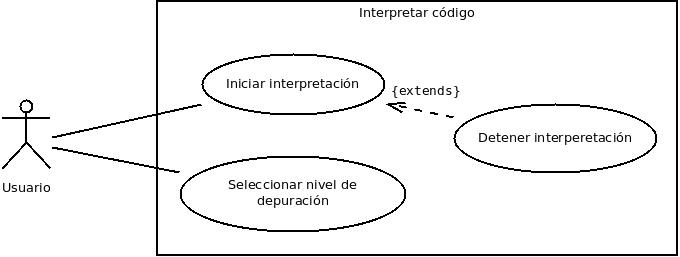
\includegraphics[width=0.9\textwidth]{./imagenes/cu2}\label{cu2}
      \caption{Caso de uso 2.- Interpretar código.}
   \end{center} \end{figure}


   \begin{table}[!ht] %% Tabla Caso de uso 2.1 - Iniciar intepretación.
      \centering
      \begin{tabular}{|p{4cm}|p{11.5cm}|}
      \hline
      \textbf{Caso de uso} & \textit{Iniciar interpretación.}\\ \hline
      \textbf{Objetivo} & \textit{Interpretar el código contenido en el editor y mostrar los resultados de la interpretación.}\\ \hline
      \textbf{Actores} & \textit{Usuario.}\\ \hline
      \textbf{Disparador} & \textit{Este caso de uso se dispara cuando el usuario selecciona la opción de interpretar código.}\\ \hline
      \textbf{Precondiciones} & \textit{Ninguna.}\\ \hline
      \textbf{Descripción} & \textit{Interpreta el código contenido en el editor y muestra los resultados.}\\ \hline
      \multicolumn{2}{|c|}{\textbf{Curso normal de los eventos}}\\ \hline
    \end{tabular}
    \begin{tabular}{|p{7.75cm}|p{7.75cm}|}
      \hspace{2cm}\textbf{Acción de los actores} & \hspace{1.75cm}\textbf{Respuesta del sistema}\\ \hline
            & \textit{1.- El sistema interpreta el código.} \textit{2.- El sistema carga la animación del Stickman correspondiente a la interpretación.}
               \textit{3.- El sistema muestra los mensajes correspondientes a la interpretación del código.} \\ \hline
    \end{tabular}
    \begin{tabular}{|p{15.9cm}|}
      \hspace{6cm}\textbf{Cursos alternativos}\\ \hline     
      \textit{Ninguno.} \\ \hline
    \end{tabular}
    \caption{Caso de uso 2.1.- Iniciar interpretación.}
   \end{table}


   \begin{table}[!ht] %% Tabla Caso de uso 2.2 - Detener intepretación.
      \centering
      \begin{tabular}{|p{4cm}|p{11.5cm}|}
      \hline
      \textbf{Caso de uso} & \textit{Detener interpretación.}\\ \hline  
      \textbf{Objetivo} & \textit{Detener la interpretación de código.}\\\hline
      \textbf{Actores} & \textit{Usuario.}\\ \hline
      \textbf{Disparador} & \textit{Este caso de uso se dispara cuando el usuario selecciona la opción de detener la interpretación de código
            que se está llevando a cabo.}\\ \hline
      \textbf{Precondiciones} & \textit{Para que esta caso de uso se puede llevar a cabo, el caso de uso 2.1.- Interpretar código tiene que estar
              ejecutándose.}\\ \hline
      \textbf{Descripción} & \textit{Detiene la interpretación de código que se está llevando a cabo.}\\ \hline
      \multicolumn{2}{|c|}{\textbf{Curso normal de los eventos}}\\ \hline
    \end{tabular}
    \begin{tabular}{|p{7.75cm}|p{7.75cm}|}
      \hspace{2cm}\textbf{Acción de los actores} & \hspace{1.75cm}\textbf{Respuesta del sistema}\\ \hline
            & \textit{1.- El sistema detiene la interpretación de código que se esté llevando a cabo.} \\ \hline
    \end{tabular}
    \begin{tabular}{|p{15.9cm}|}
      \hspace{6cm}\textbf{Cursos alternativos}\\ \hline     
      \textit{Ninguno.} \\ \hline
    \end{tabular}
    \caption{Caso de uso 2.2.- Detener interpretación.}
   \end{table}


   \begin{table}[!ht] %% Tabla Caso de uso 2.3 - Seleccionar nivel de depuración.
      \centering
      \begin{tabular}{|p{4cm}|p{11.5cm}|}
      \hline
      \textbf{Caso de uso} & \textit{Seleccionar nivel de depuración.}\\ \hline 
      \textbf{Objetivo} & \textit{Establecer el nivel de depuración que se llevará a cabo durante la siguiente interpretación.}\\ \hline
      \textbf{Actores} & \textit{Usuario.}\\ \hline
      \textbf{Disparador} & \textit{Este caso de uso se dispara cuando el usuario selecciona la opción correspondiente para seleccionar el nivel de
            depuración.}\\ \hline
      \textbf{Precondiciones} & \textit{Ninguna.}\\ \hline
      \textbf{Descripción} & \textit{Establece el nivel de depuración para la siguiente interpretación.}\\ \hline
      \multicolumn{2}{|c|}{\textbf{Curso normal de los eventos}}\\ \hline
    \end{tabular}
    \begin{tabular}{|p{7.75cm}|p{7.75cm}|}
      \hspace{2cm}\textbf{Acción de los actores} & \hspace{1.75cm}\textbf{Respuesta del sistema}\\ \hline
      \textit{2.- El usuario selecciona el nivel de depuración deseado.} & \textit{1.- El sistema da a elegir 3 niveles de depuración al usuario:}
            \textit{  - Sólo errores.} \textit{  - Información básica.} \textit{  - Información auxiliar.} \textit{3.- El sistema almacena el 
            nuevo nivel de depuración.} \\ \hline
    \end{tabular}
    \begin{tabular}{|p{15.9cm}|}
      \hspace{6cm}\textbf{Cursos alternativos}\\ \hline     
      \textit{Ninguno.} \\ \hline
    \end{tabular}
    \caption{Caso de uso 2.3.- Seleccionar nivel de depuración.}
   \end{table}

